Welcome to week 3! This week, we’ll be covering logistic regression. Logistic regression is a method for classifying data into discrete outcomes. For example, we might use logistic regression to classify an email as spam or not spam. In this module, we introduce the notion of classification, the cost function for logistic regression, and the application of logistic regression to multi-class classification.

We are also covering regularization. Machine learning models need to generalize well to new examples that the model has not seen in practice. We’ll introduce regularization, which helps prevent models from overfitting the training data. 

\section{Classification and Representation}
\subsection{Hypothesis Representation}
In binary classification problem, output $y$ will only be $0$ or $1$. Using linear regression and a threshold to determine where $y = 1$ or $y = 0$ because some extreme input data can modify brutally the regression. Therefore, we need to use another hypothesis function, the \textbf{Sigmoid Function} (also called \textbf{Logistic Function}) which is defined in formula \eqref{formSigmoid}.
\begin{align} \label{formSigmoid}
	h_\theta (x) 	&=  g ( \theta^T x ) \nonumber \\
	z 				&= \theta^T x \nonumber \\
	g(z) 			&= \dfrac{1}{1 + e^{-z}}
\end{align}
\myaligns{Sigmoid Function}
The code in listing \ref{lstSigmoid} shows how to plot this function (figure \ref{figSigmoid}) in Octave.
\begin{lstlisting}[label=lstSigmoid,caption=Sigmoid Function]
z = -20:1:20;
g = 1 ./ (1 + exp(-z));
figure;
plot(z,g);
xlabel('z'); ylabel('g');
axis([-20 20 -0.5 1.5]);
\end{lstlisting}
The function $g(z)$, shown here, maps any real number to the $(0, 1)$ interval, making it useful for transforming an arbitrary-valued function into a function better suited for classification. We start with our old hypothesis (linear regression), except that we want to restrict the range to 0 and 1. This is accomplished by plugging $z = \theta^Tx$ into the Logistic Function. 
\begin{figure}[!ht]
\centering
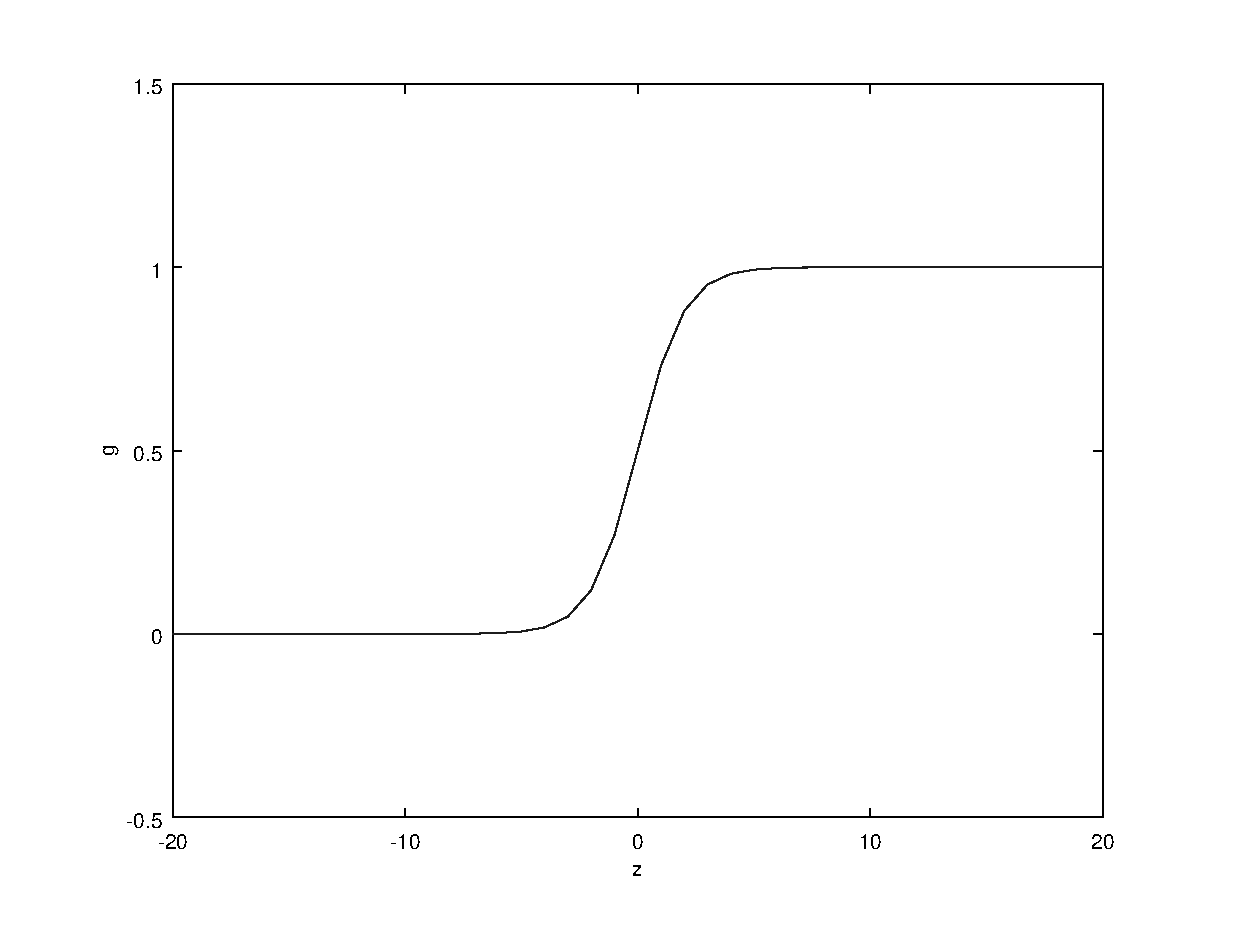
\includegraphics[scale = 0.6]{sigmoid.eps}
\caption[Sigmoid Function]{Sigmoid Function: $g = \frac{1}{1 + e^{-z}}$}
\label{figSigmoid}
\end{figure}

\subsection{Boundary Decision}
The hypothesis function $h_\theta$ gives us the probability that our output equals $1$. In binary classification, we have:
\begin{align*}
h_\theta(x) &= \mathbb{P}(y=1 | x ; \theta) = 1 - \mathbb{P}(y=0 | x ; \theta)
\end{align*} 
In order to get our discrete 0 or 1 classification, we can translate the output of the hypothesis function as follows:
\begin{align*}
& h_\theta(x) \geq 0.5 \rightarrow y = 1 \\
& h_\theta(x) < 0.5 \rightarrow y = 0
\end{align*}
From formula \eqref{formSigmoid} we deduce that:
\begin{align*}
h_\theta(x) = g(\theta^T x) \geq 0.5 \Leftrightarrow \theta^T x \geq 0
\end{align*}
which is equivalent to expression below: 
\begin{align}
& \theta^T x \geq 0 \rightarrow y = 1 \\
& \theta^T x < 0 \rightarrow y = 0 \nonumber
\end{align}
The \textbf{Boundary Decision} is the line separates the two areas $y = 0$ and $y = 1$. It can be a straight line or a circle and so on. In fact, it's the set of $x$ that satisfying formula \eqref{formBounDeci}:
\begin{align} \label{formBounDeci}
\theta^Tx = 0
\end{align}
\myaligns{Boundary Decision}

\section{Logistic Regression Model}
\subsection{Cost Function}
